%%%%%%%%%%%%%%%%%%%%%%%%%%%%%%%%%%%%%%%%%%%%%%%%%%%%%%%%%%%%%%%%%%%%%%%%%%%%%%%%
%%
%%   BornAgain User Manual
%%
%%   homepage:   http://www.bornagainproject.org
%%
%%   copyright:  Forschungszentrum Jülich GmbH 2015
%%
%%   license:    Creative Commons CC-BY-SA
%%
%%   authors:    Scientific Computing Group at MLZ Garching
%%               C. Durniak, M. Ganeva, G. Pospelov, W. Van Herck, J. Wuttke
%%
%%%%%%%%%%%%%%%%%%%%%%%%%%%%%%%%%%%%%%%%%%%%%%%%%%%%%%%%%%%%%%%%%%%%%%%%%%%%%%%%

\part{Reference}\label{PREF}
\chapter{Basics}\label{SRefBas}

This Reference is organized top-down: We start with top-level classes like
\texttt{GISAS\-Simulation};
then we explain the classes needed to set up a meaningful simulation.
For an alphabetic lookup of classes and functions,
see the general Index at the end of this Manual.
For classes and functions not explained here,
see the automatically generated Doxygen documentation.

%%%%%%%%%%%%%%%%%%%%%%%%%%%%%%%%%%%%%%%%%%%%%%%%%%%%%%%%%%%%%%%%%%%%%%%%%%%%%%%%
\section{Simulation classes}\label{SRefSim}
%%%%%%%%%%%%%%%%%%%%%%%%%%%%%%%%%%%%%%%%%%%%%%%%%%%%%%%%%%%%%%%%%%%%%%%%%%%%%%%%

Each BornAgain simulation is run from one of the three
foundational simulation classes:\footnote
{Developer note: They all inherit from a common non-public (pure virtual)
interface class \ttIdx{Simulation}.}
\ttIdx{GISAS\-Simulation},
\ttIdx{OffSpecularSimulation},
\ttIdx{SpecularSimulation}.

%===============================================================================
\subsection{GISAS\-Simulation}
%===============================================================================

Class \ttIdx{GISAS\-Simulation} controls one
grazing-incidence small-angle scattering simulation.
The following six functions from the C$++$ API are sufficient to set up and run a basic
simulation:
\setCpp
\begin{lstlisting}
class GISASSimulation {
  GISASSimulation(); // constructor
  void setDetectorParameters(...);
  void setBeamParameters(...);
  void setSample(...);
  void runSimulation();
  Histogram2D* getIntensityData(...);
};
\end{lstlisting}
\constrHide{GISAS\-Simulation}%
They shall now be explained with full signatures.
Some alternatives will also be shown.

%--------------------------------------------------------------------------------
\begin{figure}[tb]
\begin{center}
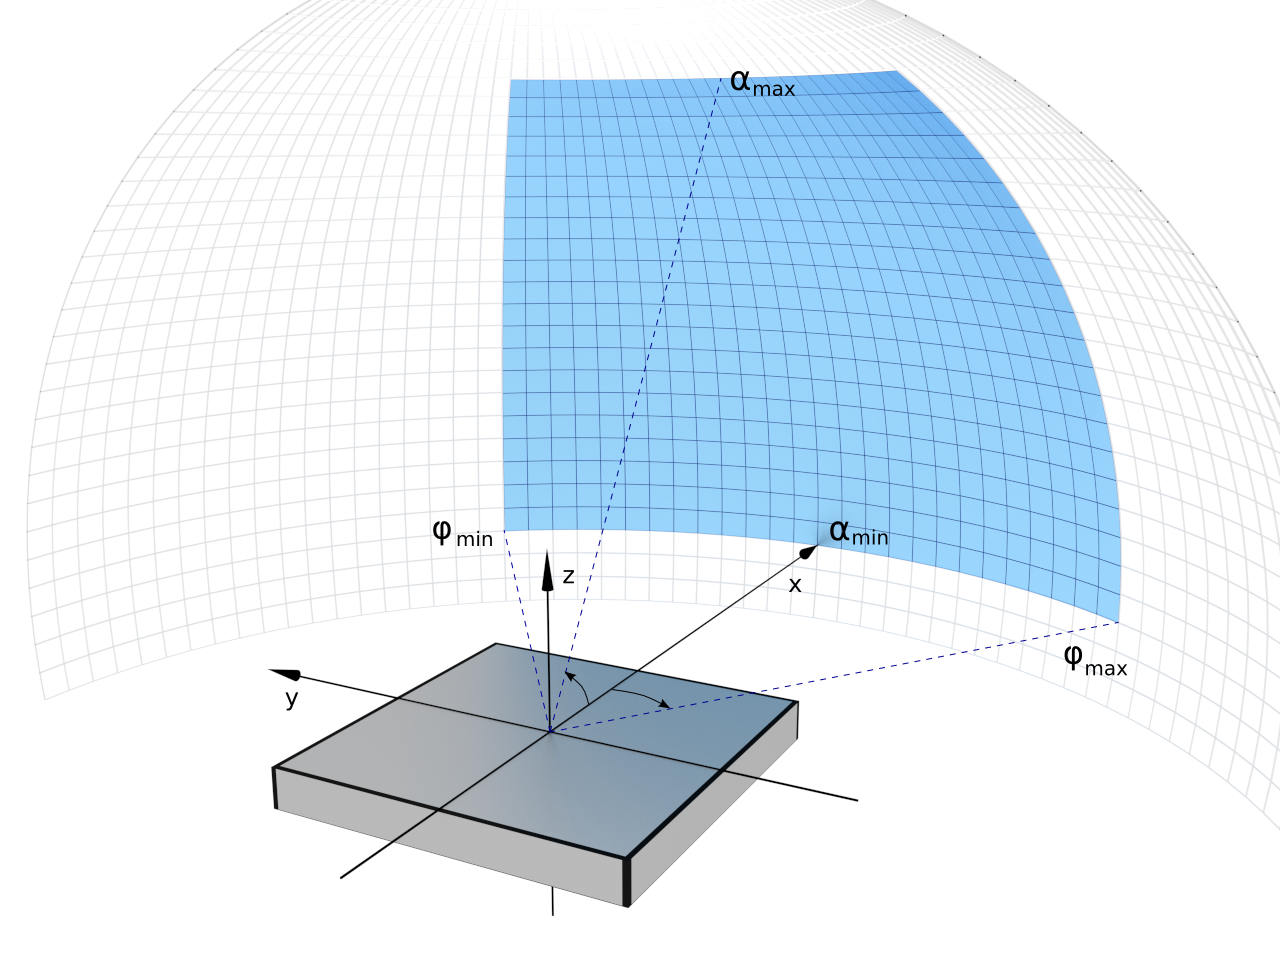
\includegraphics[width=0.7\textwidth]{fig/drawing/gisas_spherical_detector.png}
\end{center}
\caption{A spherical detector, with geometric conventions for polar angles~$\alpha$
and azimuthal angles~$\varphi$}
\label{FDetSpher}
\end{figure}
%--------------------------------------------------------------------------------

A two-dimensional detector must be defined through on of the following calls:

\subsubsection{Detector setup}
\begin{lstlisting}
class GISASSimulation {
  void setDetectorParameters(
    size_t n_phi,   double phi_min,   double phi_max,
    size_t n_alpha, double alpha_min, double alpha_max);
  void setDetector(const IDetector2D& detector);
};
\end{lstlisting}
The function \clFct{GISAS\-Simulation}{setDetectorParameters}
defines a \ttIdx{SphericalDetector}
\index{Detector!spherical}%
with \texttt{n\_phi} equidistant azimuthal ($xy$, horizontal, off-specular) bins
\index{Azimuthal angle}%
\index{Horizontal angle}%
\index{Off-specular angle}%
\index{Angle!azimuthal ($=$ horizontal)}%
and  \texttt{n\_alpha} equidistant polar ($xz$, vertical, specular) bins (\cref{FDetSpher}).
\index{Polar angle}%
\index{Vertical angle}%
\index{Specular angle}%
\index{Angle!polar ($=$ vertical)}%

The alternate function~\clFct{GISAS\-Simulation}{setDetector}
allows to supply any detector that realizes the interface \ttIdx{IDetector2D}.
Besides \texttt{SphericalDetector}, this can be a \ttIdx{Rectangular\-Detector}.
For details, see the \tuto{141}{rectangular detector tutorial}.

\subsubsection{Beam setup}
\begin{lstlisting}
class GISASSimulation {
  void setBeamParameters(
    double wavelength, double alpha_i, double phi_i);
};
\end{lstlisting}
This function\clFctHide{GISAS\-Simulation}{setBeamParameters}
is rather self-explanatory.
The incident radiation wavelength must be given in the same length unit
that is also used in the sample description.

\subsubsection{Sample setup}
\begin{lstlisting}
class GISASSimulation {
  GISASSimulation(const MultiLayer& p_sample);
  GISASSimulation(const std::shared_ptr<IMultiLayerBuilder> p_sample_builder);
  void setSample(const MultiLayer& sample);
  void setSampleBuilder(const std::shared_ptr<IMultiLayerBuilder> p_sample_builder);
};
\end{lstlisting}
Besides function \clFct{GISAS\-Simulation}{setSample}, there is an alternate
function \clFct{GISAS\-Simulation}{setSampleBuilder}.
Either function call can be replaced by an extend forms of the constructor
\constr{GISAS\-Simulation}.

Since BornAgain is only concerned with multilayer samples,
the \E{sample} class
\index{Sample (class)|see{MultiLayer@\Code{MultiLayer}}}%
is called \ttIdx{MultiLayer},
and each \E{sample builder} must realize the interface \ttIdx{IMulti\-Layer\-Builder}.
\index{Sample builder (interface)|see{IMultiLayerBuilder@\Code{IMultiLayerBuilder}}}%

A sample builder provides a more versatile way to define a sample.
Usage examples can be found in the test cases in \ttIdx{Core/StandardSamples}
and in the Python example \ttIdx{FitSpheresInHexLattice\_builder.py}.

\subsubsection{Execution}
\begin{lstlisting}
class GISASSimulation {
  void runSimulation();
};
\end{lstlisting}
\clFctHide{GISAS\-Simulation}{runSimulation}%
Once the simulation is fully set up, it is run once through this command.
Results are stored in a protected class variable.

\subsubsection{Retrieval of result}
\begin{lstlisting}
class GISASSimulation {
  Histogram2D* getIntensityData(IDetector2D::EAxesUnits units_type = IDetector2D::DEFAULT) const;
};
\end{lstlisting}
\clFctHide{GISAS\-Simulation}{getIntensityData}%
This function returns a pointer to a \ttIdx{Histogram2D}
that contains the outcome of the simulation.

%===============================================================================
\subsection{Off\-Specular\-Simulation}
%===============================================================================

\MissingSection

%===============================================================================
\subsection{Specular\-Simulation}
%===============================================================================

\MissingSection
